% statistics_and_probability:x10 GDC:NO
\begin{question}
  \medskip
  \hspace*{\fill} [Note maximale: TBD]\par
  \medskip
  \noindent Les poids des enfants d’un groupe sont normalement distribués avec une moyenne de 22,5 kg
  et un écart-type de 2,2 kg.\par
  \medskip  

  (a) Donnez la probabilité qu’un enfant choisi au hasard ait un poids supérieur à 25,8 kg.\hspace*{\fill} [TBD]\par
  \medskip  

  (b) 95\% des enfants de ce groupe pèsent moins de k kilogrammes. Trouvez la valeur de k.\hspace*{\fill} [TBD]\par
  \medskip  

  (c) La figure ci-dessous représente une courbe normale.\par
  \hspace{1em}Sur cette figure, hachurez la région qui représente l’information suivante :\par
  \hspace{1em}87\% des enfants pèsent moins de 25 kg.\hspace*{\fill} [TBD]\par
  \medskip
  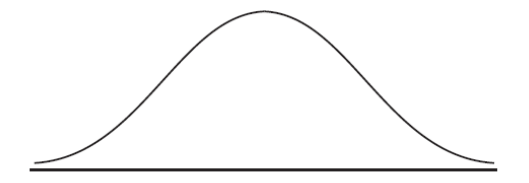
\includegraphics[scale=0.5]{courbe_normale_poids_enfants}\par  
  \medskip
\end{question}

